\documentclass[12pt]{article}
\usepackage[utf8]{inputenc}
\usepackage{graphicx}
\usepackage{amsmath}
\usepackage{hyperref}
\usepackage{amsfonts}
\usepackage{amssymb}
\usepackage{graphicx}
\usepackage{listings}
\usepackage{color}
\usepackage[left=1in,right=1in,top=1in,bottom=1in]{geometry}

\title{Rotacrypt: Rotational Mechanics as a Cryptographic Primitive}
\author{Teo Honda Scully}
\date{}

\begin{document}

\maketitle

\begin{abstract}
...TBD...
\end{abstract}

\tableofcontents

\newpage

\section{Introduction}
<...>

\subsection{Review of Rubik's Cubes}
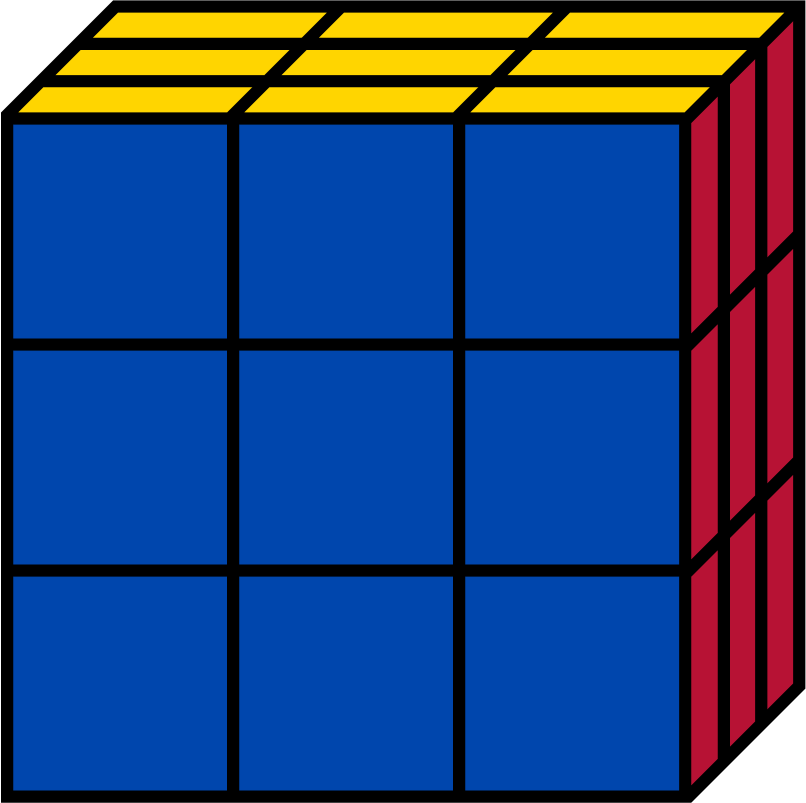
\includegraphics[scale=0.1]{cube.png}
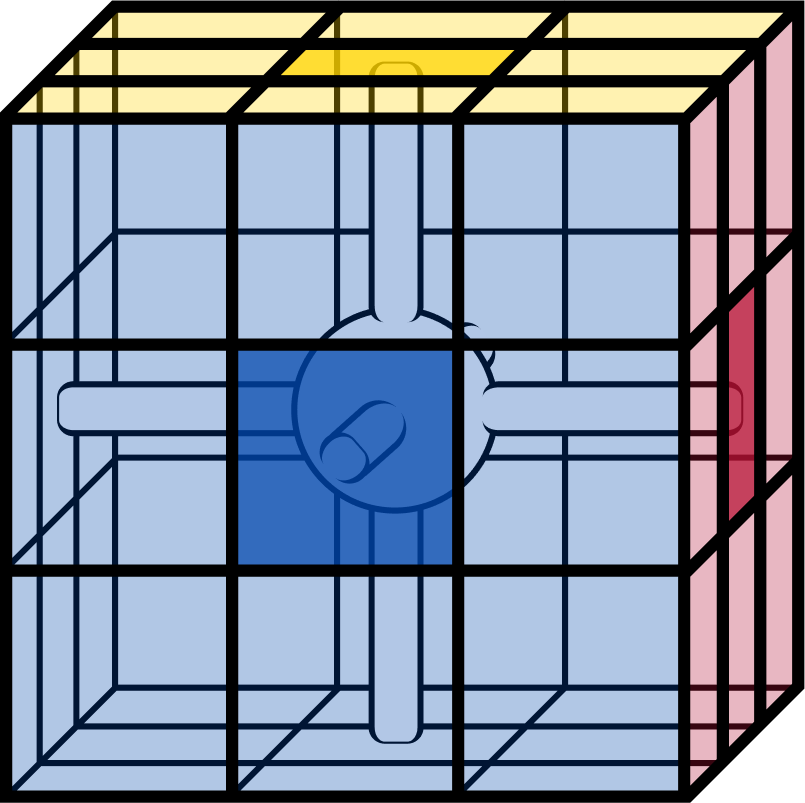
\includegraphics[scale=0.1]{core.png}

\subsection{Scheme Overview}
<...>

\subsection{Intended Usage}
<...>

\section{3x3x3 Implementation}
<...>

\subsection{Data Structure Breakdown}
<...>

\subsection{Augmented SPEFFZ Mapping}
<...>

\subsection{Cyclic Transformations}

\section{Key Generation}
<...>

\subsection{4-Cube Initialization}
<...>

\subsection{Master-Key Serialization}
<...>

\subsection{Sub-Key Generation}
<...>

\section{Encryption}
<...>

\subsection{Plaintext Setup With S-Box Transformations On Chunks}
<...>

\subsection{Cube Mapping Procedure}
<...>

\subsection{Encryption Algorithm}
<...>

\section{Decryption}
<...>

\end{document}
